\section{Patterns 2 - GoF Observer}

\subsection{Fokuspunkter}

\begin{itemize}
	\item Redegør for, hvad et Software Design Pattern er.
	\item Redegør for opbygningen af GoF Observer.
	\item Sammenlign de forskellige varianter, af GoF Observer - hvilken vil du anvende hvornår?
	\item Redegør for, hvordan anvendelsen af GoF Observer fremmer godt software design.
	\item Redegør for fordele og ulemper ved anvendelsen af GoF Observer.
	\item Redegør for, hvilke(t) SOLID-princip(per) du mener anvendelsen af GoF Observer undersøtter.
\end{itemize}

\subsection{Hvad er et Software pattern?}

\derp

\subsection{Redegør for opbygningen af GoF Observer}
\textit{"Define a one-to-many dependency between objects so that when one object changes state, all its dependents are notified and updated automatically"}\\

Opbygningen kan ses på figur~\ref{fig:observer_classdiagram} side \pageref{fig:observer_classdiagram}, som viser et klassediagram for opbygning af dette pattern.

\begin{figure}[h]
	\centering
	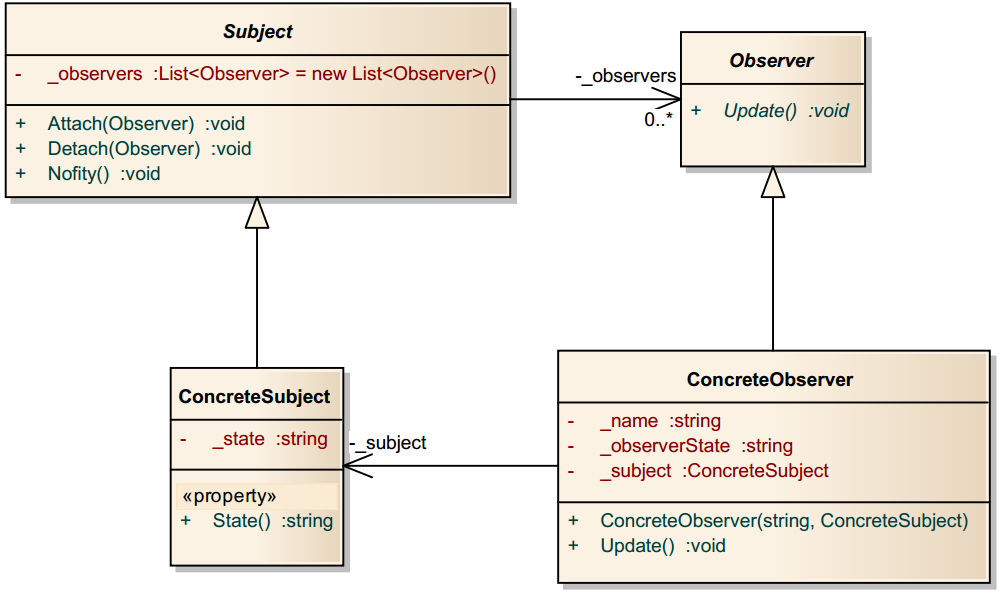
\includegraphics[width=\linewidth]{figs/observer_classdiagram}
	\caption[GoF Observer klassediagram]{Klassediagram som viser GoF Observers opbygning.}
	\label{fig:observer_classdiagram}
\end{figure}


\subsection{Sammenlign de forskellige varianter, af GoF Observer - hvilken vil du anvende hvornår?}

\subsection{Redegør for, hvordan anvendelsen af GoF Observer fremmer godt software design}

\subsection{Redegør for fordele og ulemper ved anvendelsen af GoF Observer}


\subsection{Redegør for, hvilke(t) SOLID-princip(per) du mener anvendelsen af GoF Observer undersøtter}

\begin{itemize}
	\item SRP.\\
	Ikke relevant. Alternativt er den overholdt da klasserne kun har én grund til at ændre sig.
	\item OCP.\\
	Overholdt da vi let vil kunne tilføje flere observers uden at skulle ændre i subject eller anden kode.
	\item LSP.\\
	Brud(?), da man ikke kan udskifte de nedarvede klasser med deres parent.\todo{relevant? Det er jo ikke meningen at dette overhovedet skal kunne gøres?}
	\item ISP.\\
	Overholdt(?), ikke lavet med interface i vores eksempel. Hvis det var gjort med interfaces ville disse være små og lette. 
	\item DIP.\\
	Ikke relevant, da \todo{how to explain?}
\end{itemize}